\section{Résultats}

\subsection{Suivi de la petite faune}

\subsubsection{Pièges photographiques}
Un total de \mbox{1 003 984} images enregistrées en 2024 sur l'A10 et la route 104 ont été traitées par MegaDetector, nécessitant \mbox{2 569 394} secondes de temps de calcul, ce qui correspond à 29.7 jours de calcul en continu. MegaDetector a étiqueté 62 419 objets qui étaient possiblement des animaux, en se basant sur le seuil $\geq 0.75$. Toutes ces images ont été validées par un humain et ont révélé un faible taux de vrais positifs de 3.5\%: 2 201 des détections étaient de vraies détection d'animaux. Le taux de faux positifs était de 96.5\% (i.e., détections présumées par MegaDetector mais non avérées). Ce nombre suprenant de faux positifs était associé à la fausse identification d'un ponceau par MegaDetector pour la caméra au site CAN2 sur l'A10. En effet, 54 367 fausses détections provenaient de ce site, ce qui a fait gonfler substantiellement le nombre de faux positifs. Ceci souligne l'importance d'entraîner un outil qui est adapté au contexte routier. À partir des 62 419 images étiquetées par MegaDetector, nous avons également noté des faux-négatifs, c'est-à-dire, des animaux qui n'avaient pas été détectés par MegaDetector. L'inspection de ces images a révélé 1 199 animaux additionnels. Ainsi, un total de 3 400 détections animales ont été répertoriées sur les 1 003 984 images.

Différents groupes et espèces ont été observées sur les images, incluant des invertebrés (araignées, odonates, papillons) et plusieurs vertébrés (Tableau \ref{tab:cam-sp-2024}). Des 3 400 détections animales, 42,6\% étaient de la sauvagine, 29,5\% étaient des mammifères de moyenne taille et 13\% étaient des anoures. Les autres animaux détectés étaient des oiseaux forestiers (10\%), des cerfs de Virginie (5\%) et des petits mammifères (0.7\%) (Fig. \ref{fig:cam-Prop-2024}. Certains groupes, comme les anoures et la sauvagine semblaient être plus fréquents à proximité de l'A10 que la route 104, mais ceci pourrait découler de l'emplacement des caméras qui avaient été choisis (Fig. \ref{fig:cam-Prop-Type-2024}). En effet, plusieurs caméras de la route 104 étaient installées à proximité ou directement sous un pont.

\begin{table}
  \caption{Espèces et groupes d'espèces répertoriées sur les images prises par les pièges photographiques à proximité de ponceaux ou passages potentiels sur l'A10 et la route 104 en 2024. Le tableau a été préparé à partir des 3 400 détections animales.}
  \label{tab:cam-sp-2024}
  \begin{tabular}{p{0.3\textwidth}p{0.7\textwidth}}
    \hline
    Groupe & Espèces ou niveau taxonomique supérieur \\
    \hline
    Amphibiens & Anoures (\emph{Lithobates} sp.) \\
    Oiseaux forestiers & Passereaux et rapaces \\
    Sauvagine & Canards, bernaches (\emph{Branta canadensis}) et échassiers (grand héron \emph{Ardea herodias}, grande aigrette \emph{Ardea alba}) \\
    Petits mammifères & Écureuil roux (\emph{Tamiasciurus hudsonicus}), écureuil gris (\emph{Sciurus carolinensis}), souris (\emph{Zapus hudsonius} ou \emph{Napaeozapus insignis}), campagnols (\emph{Microtus pennsylvanicus} ou \emph{Clethrionomys gapperi}) \\
    Mammmifères moyens & castor du Canada (\emph{Castor canadensis}), chat domestique (\emph{Felis catus}), lièvre d’Amérique (\emph{Lepus americanus}), loutre de rivière (\emph{Lontra canadensis}), marmotte commune (\emph{Marmota monax}), mouffette rayée (\emph{Mephitis mephitis}), \emph{Mustela} sp., opossum de Virginie (\emph{Didelphis virginiana}), raton laveur (\emph{Procyon lotor}, rat musqué (\emph{Ondatra zibethicus}), renard roux (\emph{Vulpes vulpes}) \\
    Grands mammifères & Cerf de Virginie (\emph{Odocoileus virginianus}) \\
    Invertébrés & Araignées, abeilles, lépidoptères, odonates et escargots \\
   \hline
  \end{tabular}
\end{table}


\begin{figure}
  \centering
  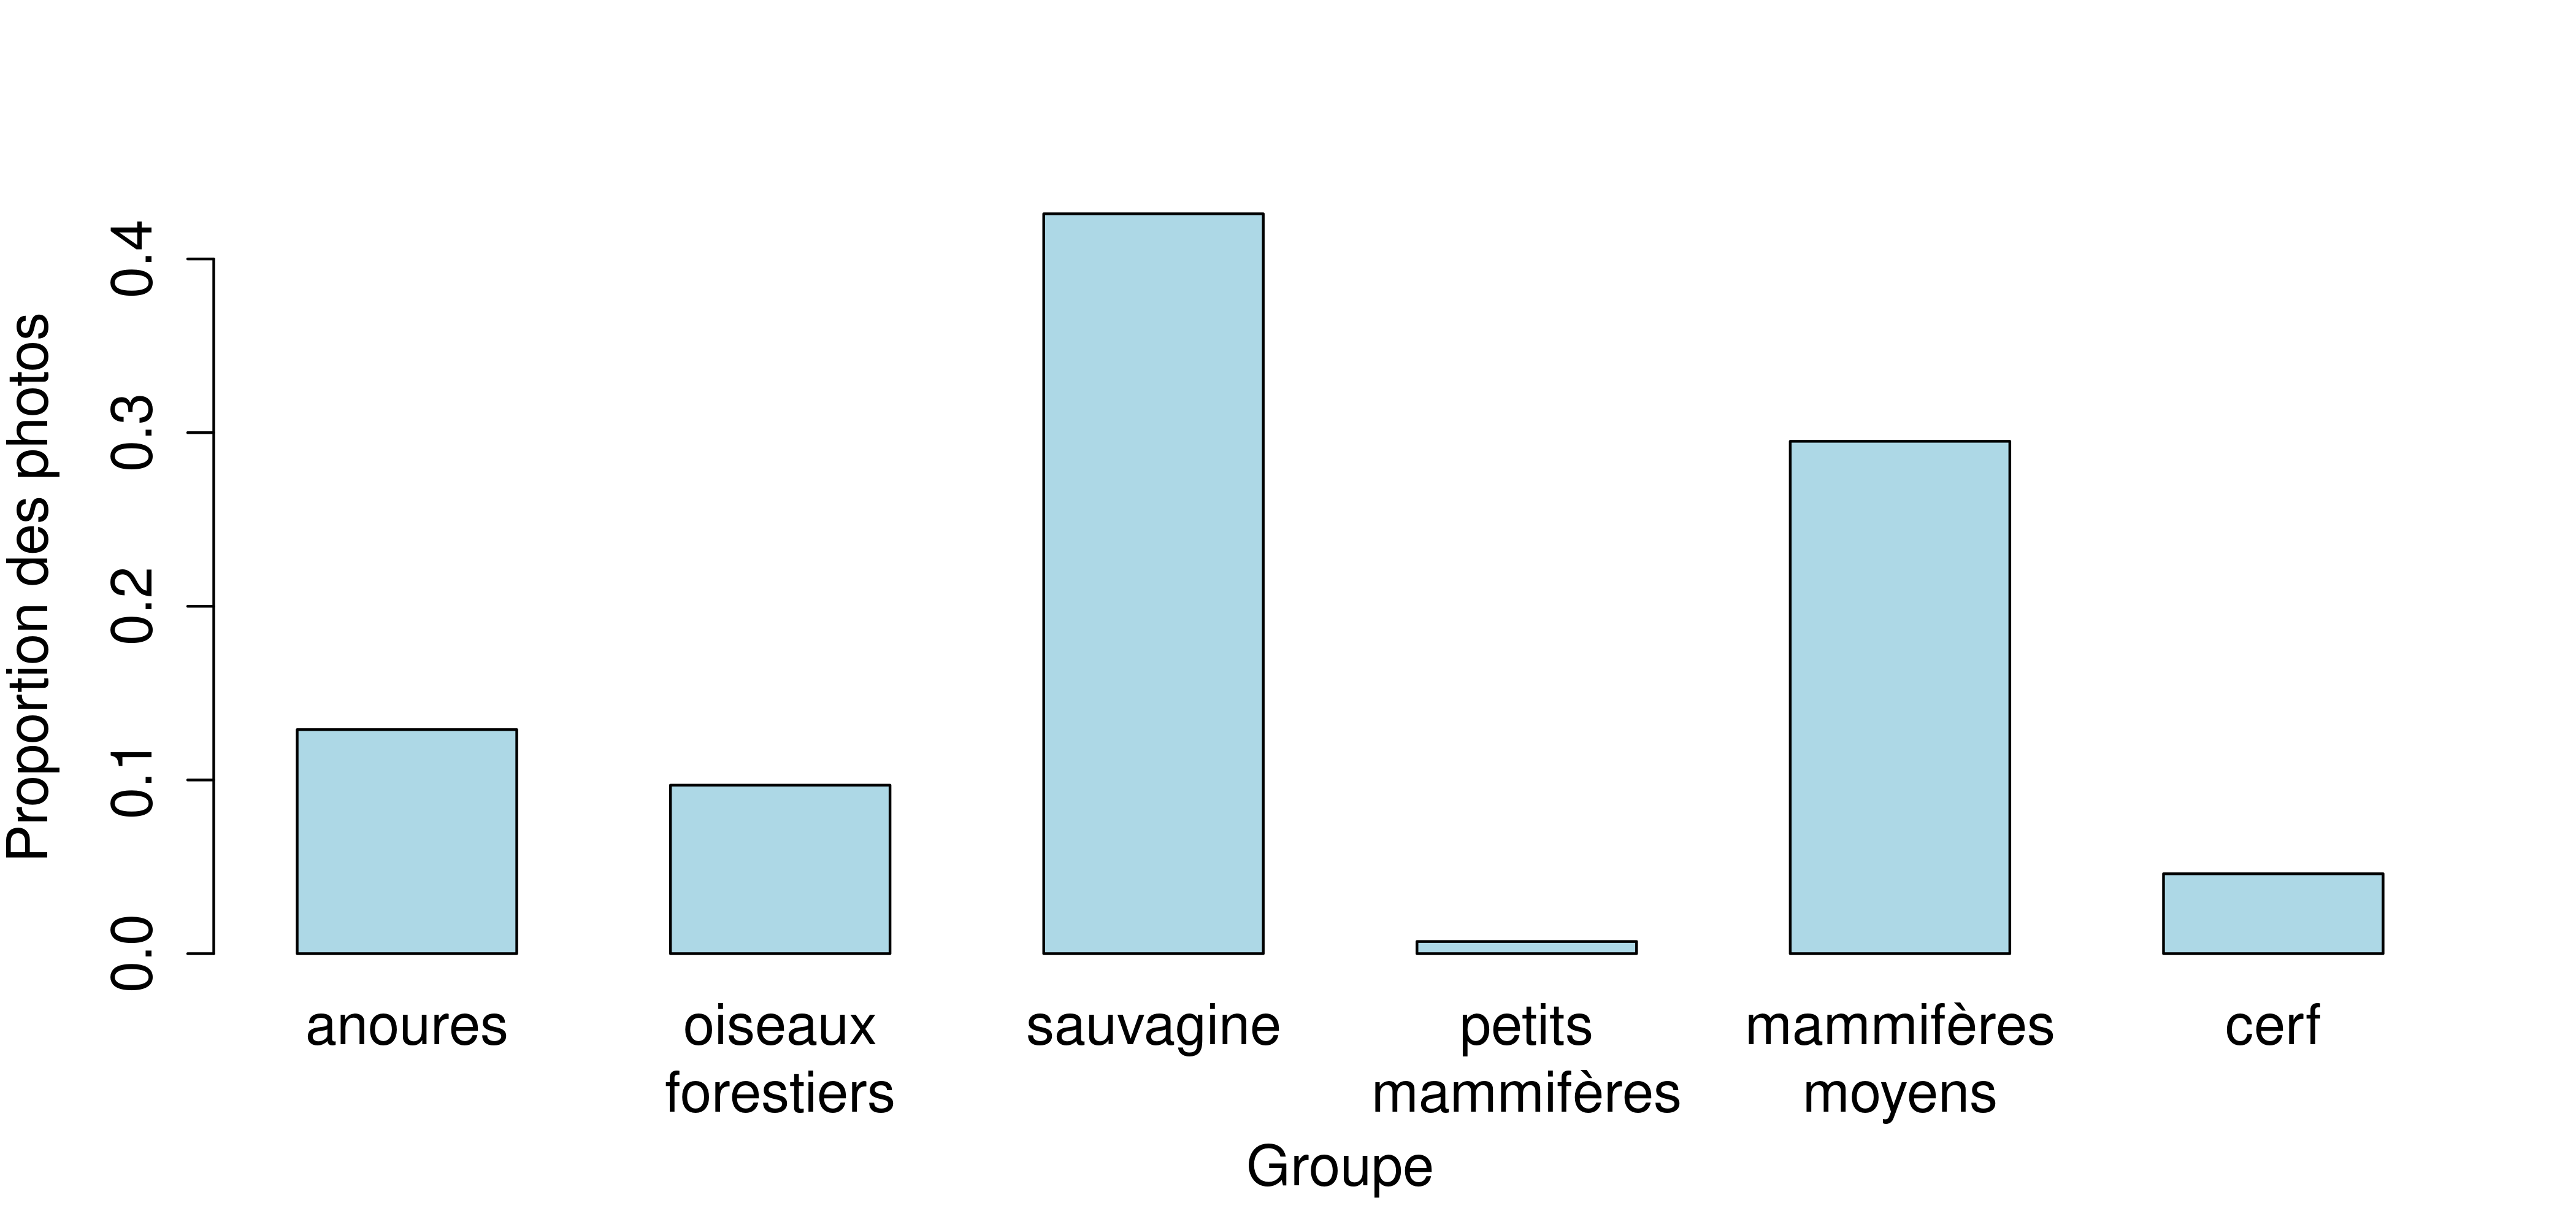
\includegraphics[width=0.9\textwidth]{fig/cam-Prop-2024.png}
\caption{Proportions des images avec détection animales de vertébrés prises par les pièges photographiques à proximité de ponceaux ou passages potentiels sur l'A10 et la route 104 en 2024. La figure a été préparée à partir des 3 400 détections animales.}
\label{fig:cam-Prop-2024}
\end{figure}


\begin{figure}
  \centering
  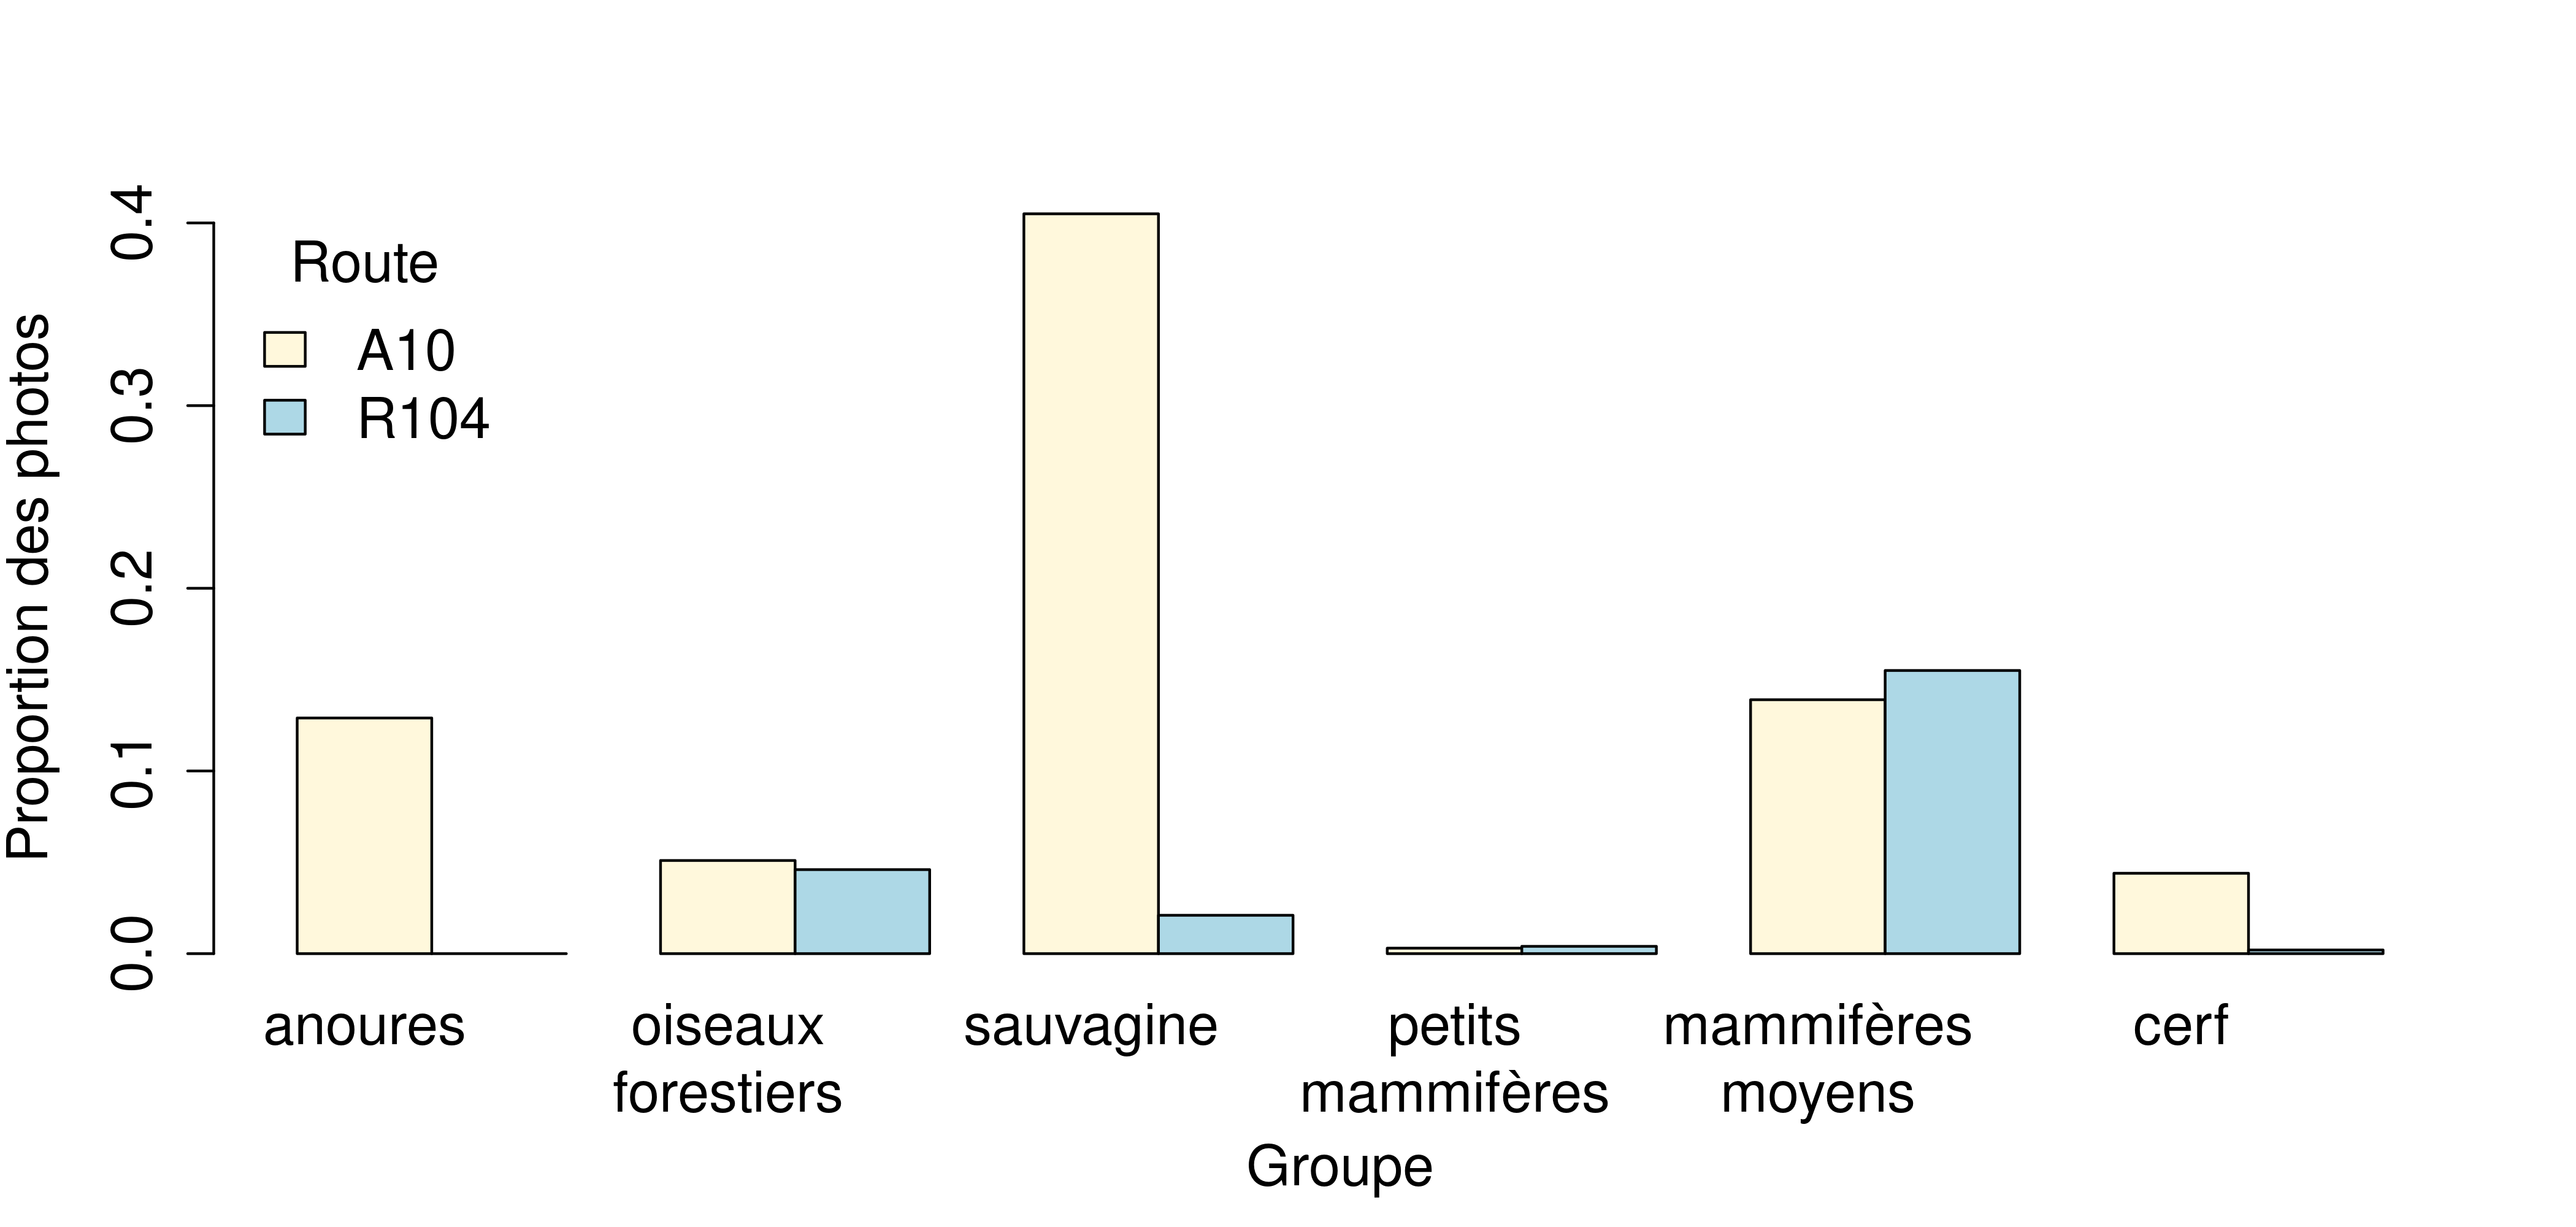
\includegraphics[width=0.9\textwidth]{fig/cam-Prop-Type-2024.png}
\caption{Proportions des images avec détection animales de vertébrés prises par les pièges photographiques dans les ponceaux à proximité de ponceaux ou passages potentiels en 2024 présentés séparément pour l'A10 et la route 104. La figure a été préparée à partir des 3 400 détections animales.}
\label{fig:cam-Prop-Type-2024}
\end{figure}
